\documentclass{beamer}
\mode<presentation>
\usetheme{CambridgeUS}
\usepackage[russian]{babel}
\usepackage[utf8]{inputenc}
\usepackage[T2A]{fontenc}
\usepackage{sansmathaccent}

\usepackage{verbatim}
\usepackage{alltt}

\pdfmapfile{+sansmathaccent.map}
\title[Шаблоны]{Шаблоны информационной архитектуры}
\author{Наумов Д.А., доц. каф. КТ}
\date[18.11.2020] {Компьютерная графика и проектирование графических интерфейсов, 2020}

\begin{document}

%ТИТУЛЬНЫЙ СЛАЙД
\begin{frame}
  \titlepage
\end{frame}
  
%СОДЕРЖАНИЕ ЛЕКЦИИ
\begin{frame}
  \frametitle{Содержание лекции}
  \tableofcontents  
\end{frame}

\section{Информационная архитектура, организация контента}

\begin{frame}[t]
	\textit{Высокоуровневая оганизация информации:}
	\begin{itemize}
		\item разделение сущностей -- отделение содержимого от физического представления;
		\item физическая структура -- представление материала на страницах.
	\end{itemize}
	
	Большинство приложений и многие веб-сайты организуются соглласно одному из нескольких следующих принципов:
	\begin{itemize}
		\item \textit{списки объектов} -- папка входящих сообщений;
		\item \textit{списки действий или задач} -- посмотреть, приобрести, продать, зарегистрироваться; 		
		\item \textit{списки тематических категорий} -- здоровье, наука, технология;		
		\item \textit{списки инструментов} -- календарь, адресная книга, блокнот.		
	\end{itemize}
	
	Любую страницу можно рассматривать с точки зрения того, что оно долнжа делать:
	\begin{itemize}
		\item отобразить едиственный объект (карта, книга, видео, игра);
		\item отобразить список объектов;
		\item предоставить возможность что-то сделать;
		\item выполнить определенную задачу.				
	\end{itemize}	

\end{frame} 

\begin{frame}[t]{Feature, Search and Browse}
	Расположите на главной странице три элемента: статья (описание), поиск и список категорий для навигации.
	\begin{figure}[h]
		\centering
		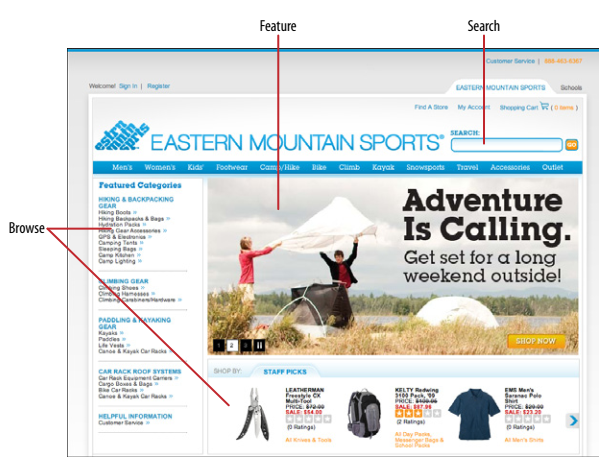
\includegraphics[scale=0.5]{images/lec07-pic01.png}
	\end{figure}
\end{frame} 

\begin{frame}[t]{Feature, Search and Browse}
	\begin{figure}[h]
		\centering
		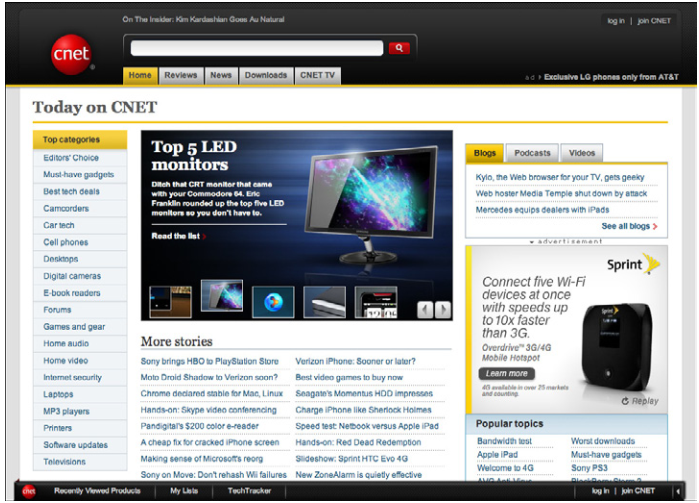
\includegraphics[scale=0.5]{images/lec07-pic02.png}
	\end{figure}
\end{frame} 

\begin{frame}[t]{News Stream}
	Отобразите элементы в обратном хронологическом порядке, обновляйте их динамически.
	\begin{figure}[h]
		\centering
		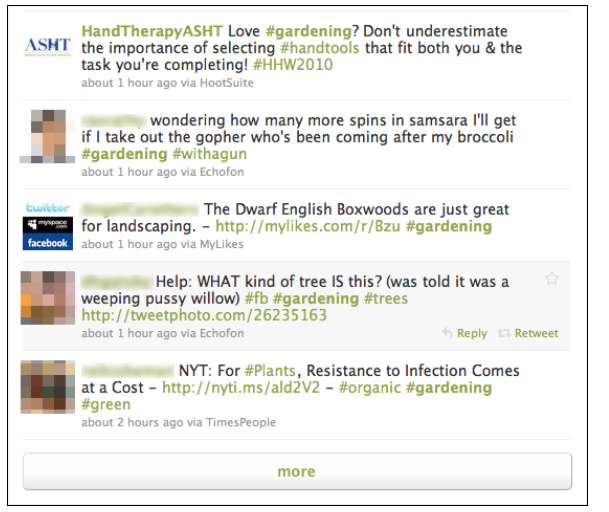
\includegraphics[scale=0.45]{images/lec07-pic04.png}
	\end{figure}
\end{frame} 

\begin{frame}[t]{Picture Manager}
	Используйте эскизы, список элементов и интерфейс просмотра.
	\begin{figure}[h]
		\centering
		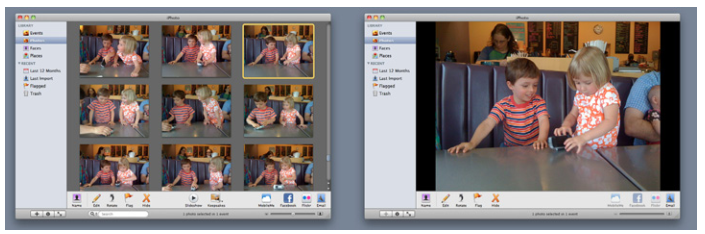
\includegraphics[scale=0.6]{images/lec07-pic06.png}
	\end{figure}
\end{frame} 

\begin{frame}[t]{Dashboard}
	Организуйте отображение данных в единую информационную страницу, регулярно обновляемую.
	\begin{figure}[h]
		\centering
		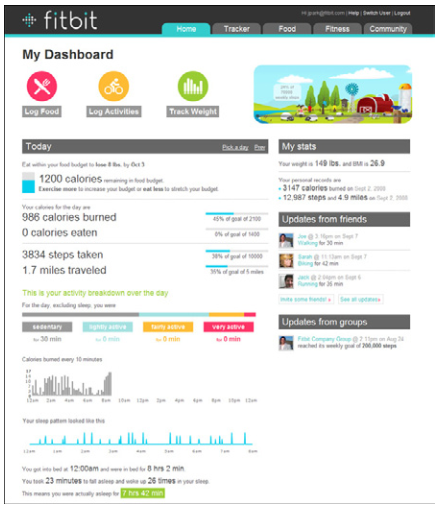
\includegraphics[scale=0.5]{images/lec07-pic08.png}
	\end{figure}
\end{frame} 

\begin{frame}[t]{Canvas plus Palette}
	Поместите палитру рядом с холстом; пользователь сможет выбирать инструменты на палитры, чтобы создать объекты на холсте.
	\begin{figure}[h]
		\centering
		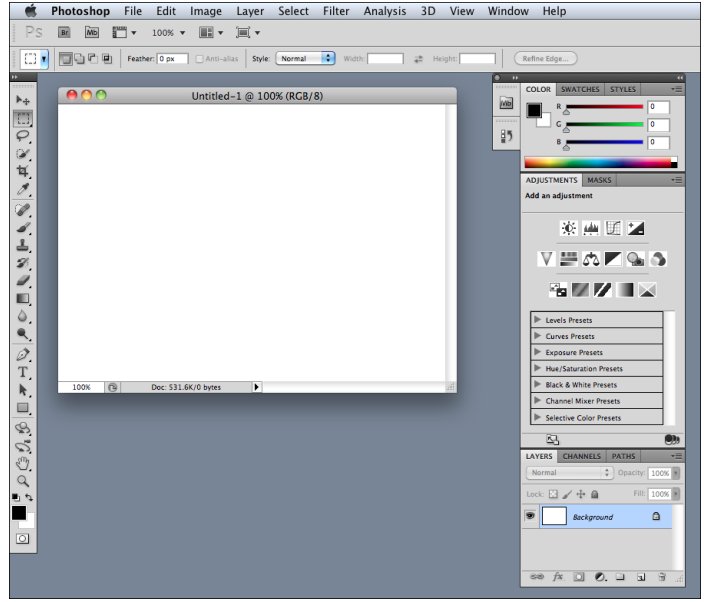
\includegraphics[scale=0.5]{images/lec07-pic09.png}
	\end{figure}
\end{frame} 

\begin{frame}[t]{Wizard}
	Проведите пользователя через интерфейс шаг за шагом, чтобы выполнить задачи в заданном порядке.
	\begin{figure}[h]
		\centering
		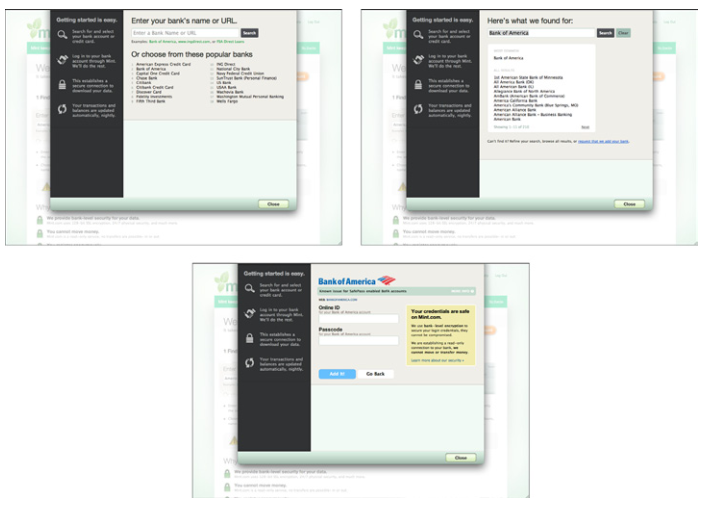
\includegraphics[scale=0.5]{images/lec07-pic10.png}
	\end{figure}
\end{frame} 

\begin{frame}[t]{Settings}
	Предоставьте легкодоступную страницу, где пользователи могут изменять настройки,
предпочтения или свойства. Разделите содержимое на отдельные вкладки или страницы, если вам нужно управлять большим количеством настроек.
	\begin{figure}[h]
		\centering
		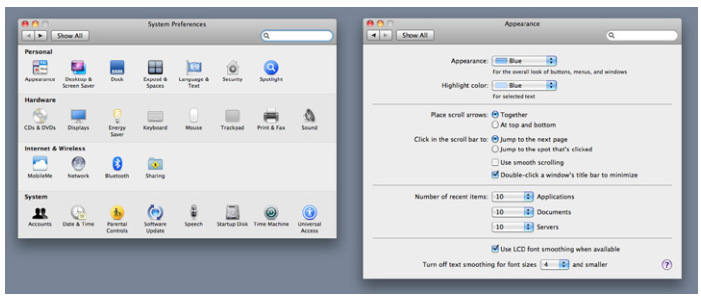
\includegraphics[scale=0.6]{images/lec07-pic11.png}
	\end{figure}
\end{frame} 

\begin{frame}[t]{Alternative Views}
	Позвольте пользователю выбирать один из альтернативных вариантов, существенно отличающихся от вида по умолчанию.
	\begin{figure}[h]
		\centering
		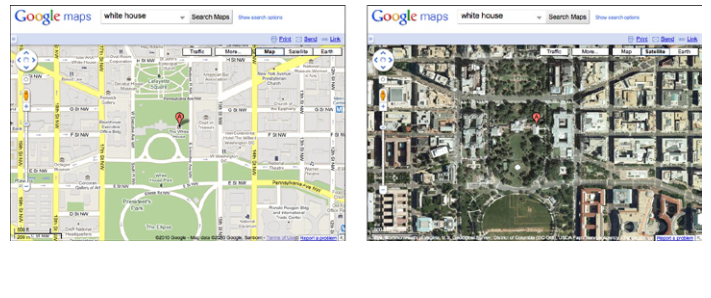
\includegraphics[scale=0.6]{images/lec07-pic12.png}
	\end{figure}
\end{frame} 

\begin{frame}[t]{Many Workspaces}
	Используйте несколько вкладок верхнего уровня, групп вкладок и окон, чтобы пользователи могли одновременно просматривать несколько страниц, проектов, файлов или контекстов. 
	\begin{figure}[h]
		\centering
		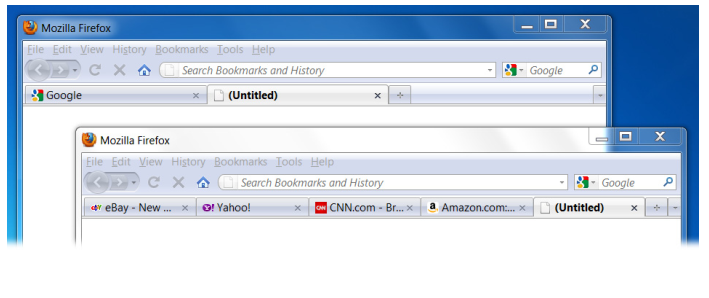
\includegraphics[scale=0.6]{images/lec07-pic13.png}
	\end{figure}
\end{frame}

\begin{frame}[t]{Multi-level Help}
	Используйте различные варианты помощи и подсказок для поддержки пользователей с различными потребностями. 
	\begin{figure}[h]
		\centering
		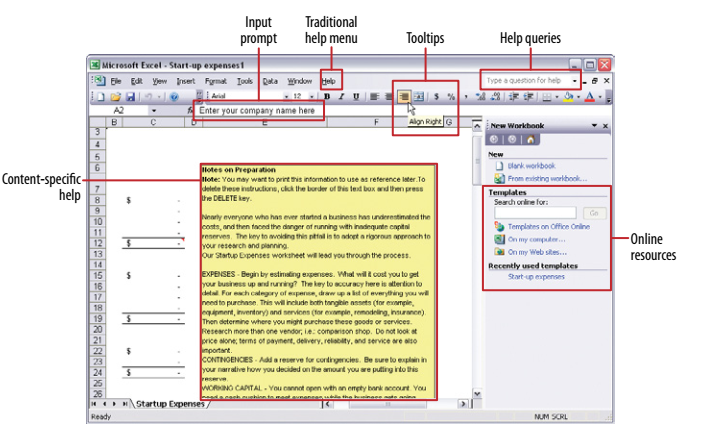
\includegraphics[scale=0.5]{images/lec07-pic14.png}
	\end{figure}
\end{frame}

\section{Навигация}

\begin{frame}
  \frametitle{Содержание лекции}
  \tableofcontents[current]
\end{frame}

\begin{frame}[t]
	Указатели (signpost) -- средства, позволяющие пользователям ориентироваться на стренице.
	\begin{itemize}
		\item заголовки (страниц, окон);
		\item логотипы;
		\item вкладки;
		\item индикаторы выбора и т.д.						
	\end{itemize}	
	Указатели:
	\begin{itemize}
		\item ясные и недвусмысленные;
		\item расположены в ожидаемом месте;
		\item создают правильную <<ментальную карту>> сайта.
	\end{itemize}
	\textit{Задача построения системы навигации}: минимизация количества переходов пользователя для достижения его целей.
	\begin{itemize}
		\item глобальная навигация;
		\item вспомогательная навигация;
		\item ассоциативная.
	\end{itemize}	
\end{frame} 

\begin{frame}[t]{Clear Entry Points}
	Представьте только несколько основных точек входа в интерфейс; сделайте их ориентированными на задачи и описательными. Используйте четкие призывы к действию. 
	\begin{figure}[h]
		\centering
		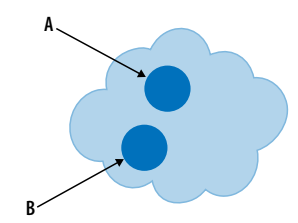
\includegraphics[scale=0.75]{images/lec07-pic23.png}
	\end{figure}
\end{frame}

\begin{frame}[t]{Clear Entry Points}
	\begin{figure}[h]
		\centering
		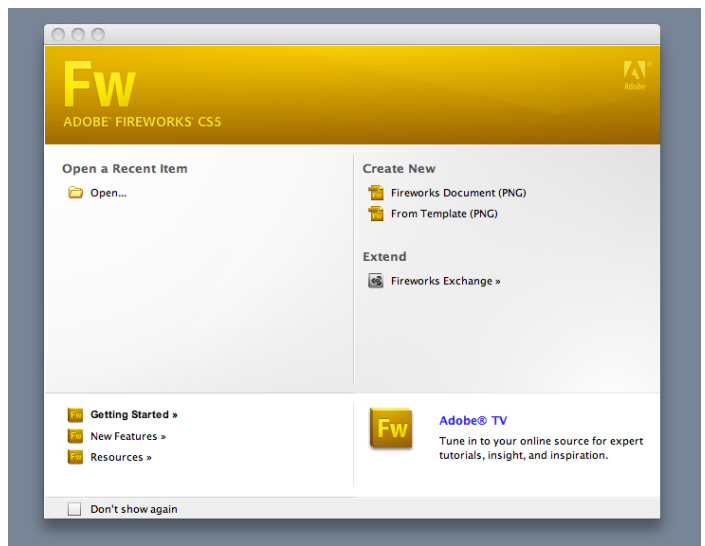
\includegraphics[scale=0.5]{images/lec07-pic24.png}
	\end{figure}
\end{frame}

\begin{frame}[t]{Main Page}
	Заполните страницу списком ссылок на содержательные страницы вашего сайта или приложения. Покажите достаточно информации о каждой ссылке, чтобы пользователь мог сделать правильный выбор. Не показывайте на странице никакого другого значимого
контента. 
	\begin{figure}[h]
		\centering
		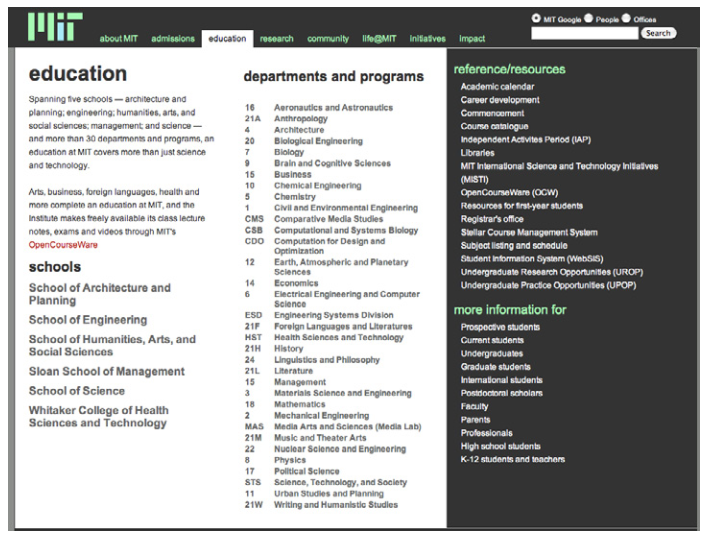
\includegraphics[scale=0.4]{images/lec07-pic26.png}
	\end{figure}
\end{frame}

\begin{frame}[t]{Main Page}
	\begin{figure}[h]
		\centering
		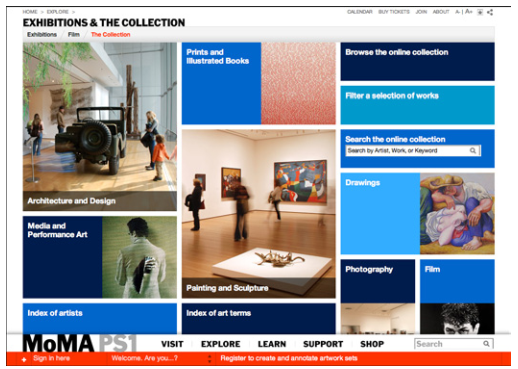
\includegraphics[scale=0.6]{images/lec07-pic27.png}
	\end{figure}
\end{frame}

\begin{frame}[t]{Pyramid}
	Создайте последовательность страниц с ссылками prev/next. Создайте родительскую страницу, которая ссылается на все страницы в этой последовательности, и позвольте пользователю просматривать их либо последовательно, либо в произольном порядке. 
	\begin{figure}[h]
		\centering
		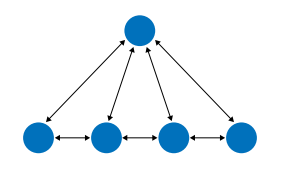
\includegraphics[scale=0.75]{images/lec07-pic28.png}
	\end{figure}
\end{frame}

\begin{frame}[t]
	\begin{figure}[h]
		\centering
		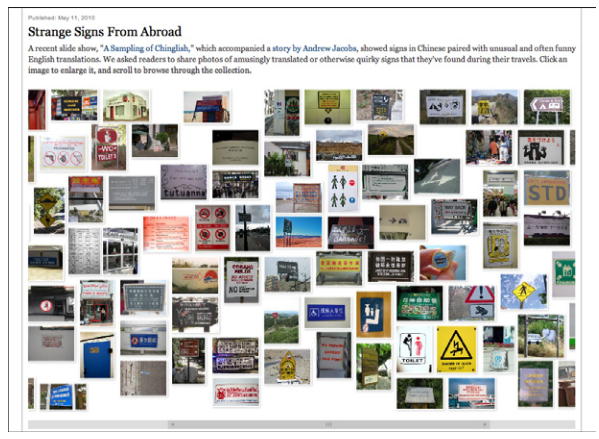
\includegraphics[scale=0.35]{images/lec07-pic29.png}
	\end{figure}
	\begin{figure}[h]
		\centering
		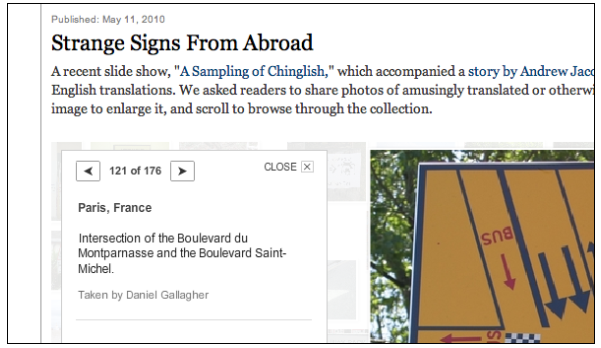
\includegraphics[scale=0.35]{images/lec07-pic30.png}
	\end{figure}
\end{frame}

\begin{frame}[t]{Modal Panel}
	Отображайте только одну страницу без каких-либо других параметров навигации, пока пользователь не выполнит ближайшую задачу. 
	\begin{figure}[h]
		\centering
		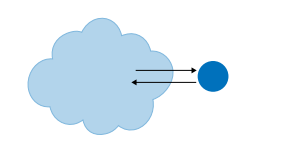
\includegraphics[scale=0.75]{images/lec07-pic31.png}
	\end{figure}
\end{frame}

\begin{frame}[t]{Modal Panel}
	\begin{figure}[h]
		\centering
		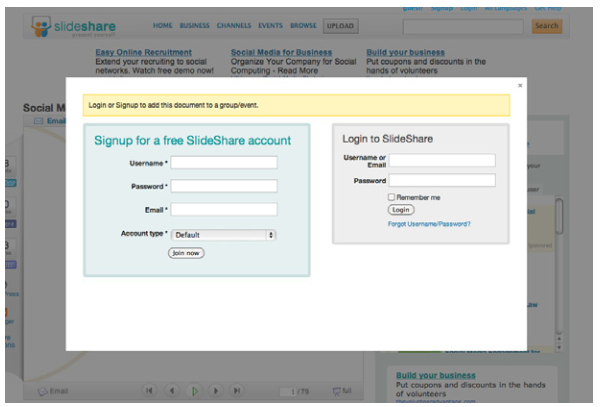
\includegraphics[scale=0.5]{images/lec07-pic32.png}
	\end{figure}
\end{frame}

\begin{frame}[t]{Deep-linked state}
	Зафиксируйте состояние сайта в URL-адресе, который можно сохранить или отправить другим людям. При загрузке он восстанавливает состояние приложения до того, что видел пользователь. 
	\begin{figure}[h]
		\centering
		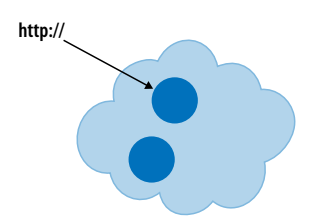
\includegraphics[scale=0.75]{images/lec07-pic33.png}
	\end{figure}
\end{frame}

\begin{frame}[t]{Deep-linked state}
	\begin{figure}[h]
		\centering
		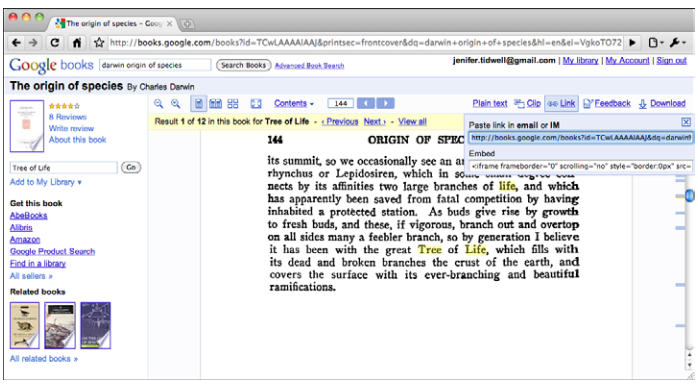
\includegraphics[scale=0.5]{images/lec07-pic34.png}
	\end{figure}
\end{frame}

\begin{frame}[t]{Escape Hatch}
	На каждом экране, имеющем ограниченные возможности навигации, поместите кнопку или ссылку, которая явно выводит пользователя из этого экрана и возвращает в известное место. 
	\begin{figure}[h]
		\centering
		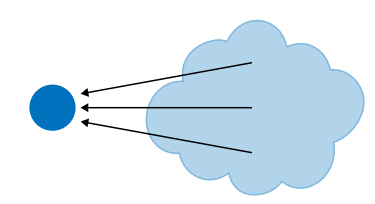
\includegraphics[scale=0.75]{images/lec07-pic35.png}
	\end{figure}
\end{frame}

\begin{frame}[t]{Escape Hatch}
	\begin{figure}[h]
		\centering
		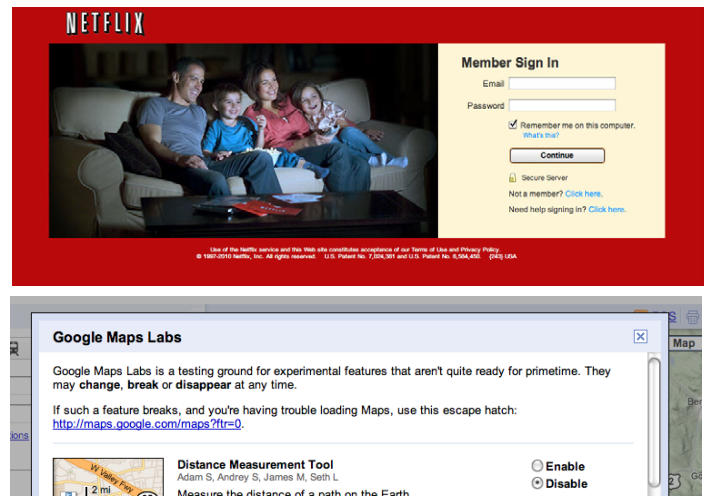
\includegraphics[scale=0.5]{images/lec07-pic36.png}
	\end{figure}
\end{frame}	

\begin{frame}[t]{Fat Menus}
	Для длинного списка навигационных ссылок используйте меню. Используйте хорошо подобранные категории или естественный порядок сортировки.
	\begin{figure}[h]
		\centering
		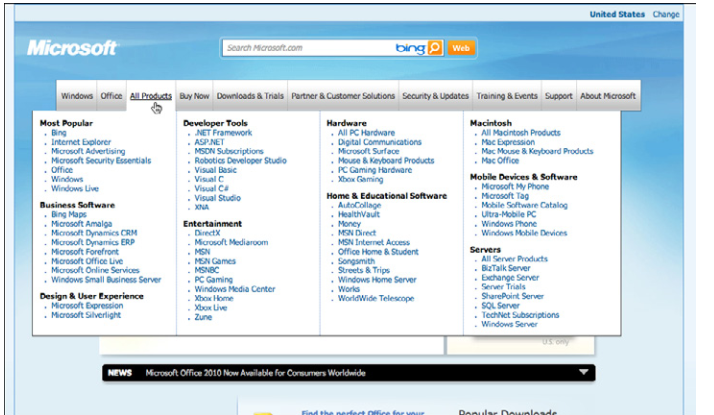
\includegraphics[scale=0.5]{images/lec07-pic37.png}
	\end{figure}
\end{frame}	

\begin{frame}[t]{Fat Menus}
	\begin{figure}[h]
		\centering
		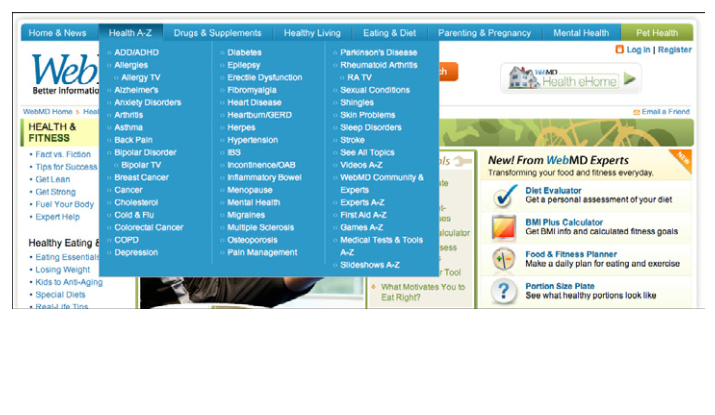
\includegraphics[scale=0.5]{images/lec07-pic38.png}
	\end{figure}
\end{frame}	

\begin{frame}[t]{Sitemap Footer}
	Поместите карту сайта в нижний колонтитул каждой страницы сайта. Рассматривайте его как часть глобальной навигации, дополняющую заголовок.
	\begin{figure}[h]
		\centering
		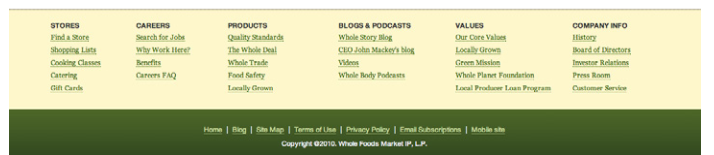
\includegraphics[scale=0.5]{images/lec07-pic39.png}
	\end{figure}
	\begin{figure}[h]
		\centering
		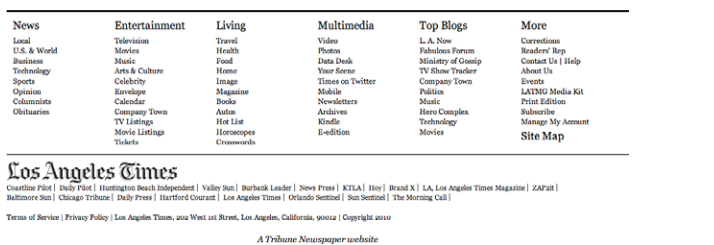
\includegraphics[scale=0.5]{images/lec07-pic41.png}
	\end{figure}	
\end{frame}	

\begin{frame}[t]{Sitemap Footer}
	\begin{figure}[h]
		\centering
		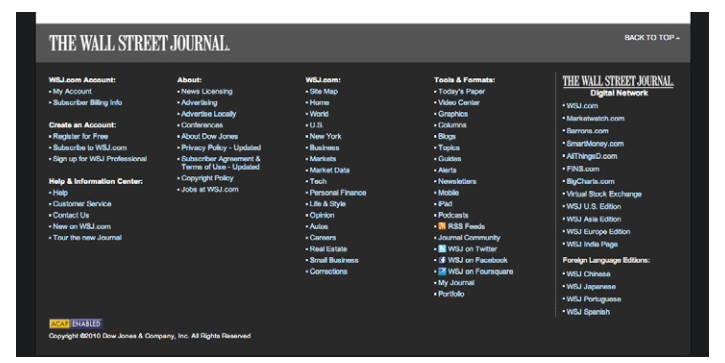
\includegraphics[scale=0.5]{images/lec07-pic40.png}
	\end{figure}	
\end{frame}	

\begin{frame}[t]{Sign-in Tools}
	Поместите служебную навигацию, связанную с регистрацией/авторизацией пользователя, в правый верхний угол. Там же расположите корзины, ссылки на настройку профиля и учетной записи, кнопки справки и выхода из системы.
	\begin{figure}[h]
		\centering
		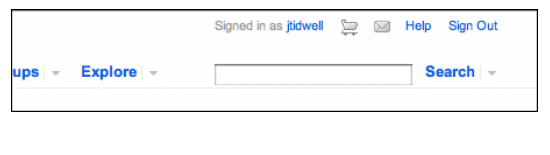
\includegraphics[scale=0.5]{images/lec07-pic42.png}
	\end{figure}
\end{frame}	

\begin{frame}[t]{Sequence Map}
	На каждой странице из определенной последовательности покажите карту всех страниц по порядку, включая индикатор <<вы находитесь здесь>>.
	\begin{figure}[h]
		\centering
		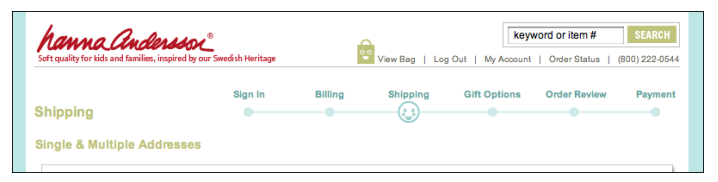
\includegraphics[scale=0.5]{images/lec07-pic43.png}
	\end{figure}
\end{frame}	

\begin{frame}[t]{Sequence Map}
	\begin{figure}[h]
		\centering
		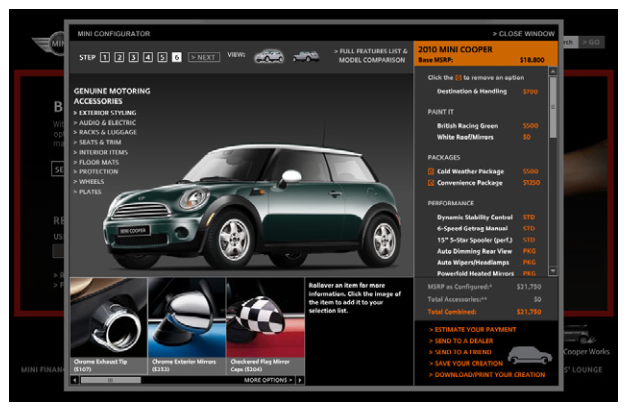
\includegraphics[scale=0.5]{images/lec07-pic44.png}
	\end{figure}
\end{frame}	

\begin{frame}[t]{Breadcrumbs}
	На каждой странице с большим количеством уровней навигационной иерархии, отображайте список всех родительских страниц, вплоть до главной или домашней страницы.
	\begin{figure}[h]
		\centering
		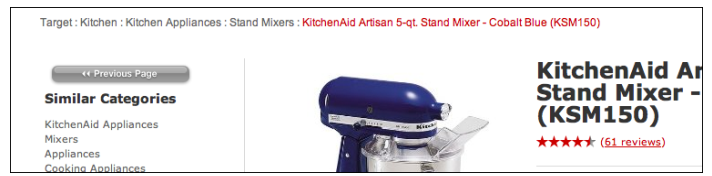
\includegraphics[scale=0.5]{images/lec07-pic45.png}
	\end{figure}
\end{frame}	

\begin{frame}[t]{Breadcrumbs}
	\begin{figure}[h]
		\centering
		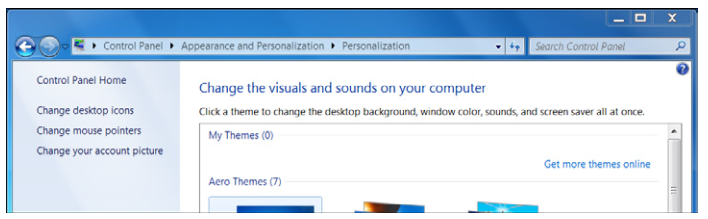
\includegraphics[scale=0.5]{images/lec07-pic46.png}
	\end{figure}
	\begin{figure}[h]
		\centering
		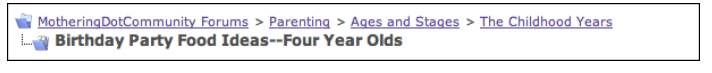
\includegraphics[scale=0.5]{images/lec07-pic47.png}
	\end{figure}	
\end{frame}

\begin{frame}[t]{Annotated Scrollbar}
	Сделайте так, чтобы полоса прокрутки могла бы использоваться в качестве индикатора <<вы здесь>>.
	\begin{figure}[h]
		\centering
		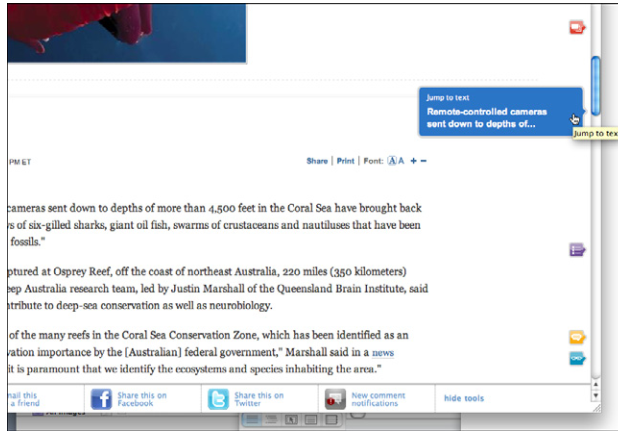
\includegraphics[scale=0.5]{images/lec07-pic48.png}
	\end{figure}
\end{frame}	

\section{Списки элементов}
\begin{frame}
  \frametitle{Содержание лекции}
  \tableofcontents[current]
\end{frame}

\begin{frame}[t]
	Как отображать списки элементов в интерактивном режиме?
	\begin{quotation}
	статьи, страницы, фото, видео,
карты, книги, игры, фильмы, сериалы, песни, средства, сообщения электронной почты, записи в блоге,
обновления статуса, сообщения на форуме, комментарии, результаты поиска, люди, события, файлы, документы,
программы, ссылки, URL-адреса, средства, способы, действия	
	\end{quotation}

	Варианты использования списков:
	\begin{itemize}
		\item получить краткий обзор всего списка;
		\item просмотреть список поэлементно;
		\item найти конретный элемент;
		\item выполнить сортировку и фильтрацию;
		\item выполнить перестановку элементов;
		\item выполнить	редактирование (добавление, удаление, изменение данных или категории).
	\end{itemize}
\end{frame}	

\begin{frame}{Характеристики списка}
	\begin{itemize}
		\item количество элементов
		\begin{itemize}
			\item поместиться ли в заданное пространство
			\item может ли быть <<бесконечным>>?			
		\end{itemize}
		\item порядок элементов		
		\begin{itemize}
			\item какая сортировка по-умолчанию
			\item необходимо ли добавить пользователю возможность сортивать список, по каким полям?
			\item нужна ли группировка элементов?			
		\end{itemize}
		\item группировка
		\begin{itemize}
			\item можно ли классифицировать элементы на категории?
			\item ... и категории - на категории более высокого уровня?
			\item может ли ползователь создавать собственные категории?
		\end{itemize}	
	\end{itemize}
\end{frame}	

\begin{frame}{Характеристики списка}
	\begin{itemize}
		\item тип элементов
		\begin{itemize}
			\item простой или сложный?
			\item элемент -- часть чего-то большего (заголовок статьи)?
			\item является ли каждый элемент структурой с набором полей?
		\end{itemize}	
		\item взаимодействие с пользователем
		\begin{itemize}
			\item отображать ли элемент целиком или по запросу?
			\item что ползователь может делать с элементом?
			\item можно ли выбирать элемент? несколько элементов?
		\end{itemize}
		\item поведение
		\begin{itemize}
			\item как долго загружается?
			\item можно ли изменять <<на лету>>? что произойдет в этом случае?
		\end{itemize}		
	\end{itemize}
\end{frame}	

\begin{frame}[t]{Two-Panel Selector}
	Поместите две боковые панели на интерфейс. В первом из них отображается список элементов, которые
пользователь может выбрать по своему желанию; во втором -- содержимое выбранного элемента.
	\begin{figure}[h]
		\centering
		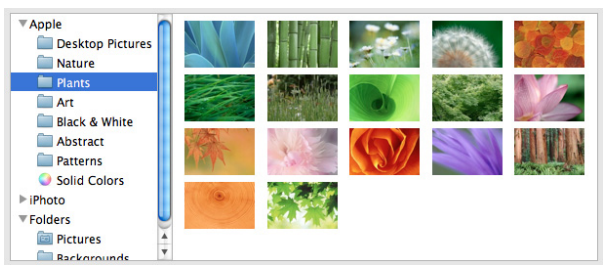
\includegraphics[scale=0.6]{images/lec07-pic49.png}
	\end{figure}
\end{frame}	

\begin{frame}[t]{Two-Panel Selector}
	\begin{figure}[h]
		\centering
		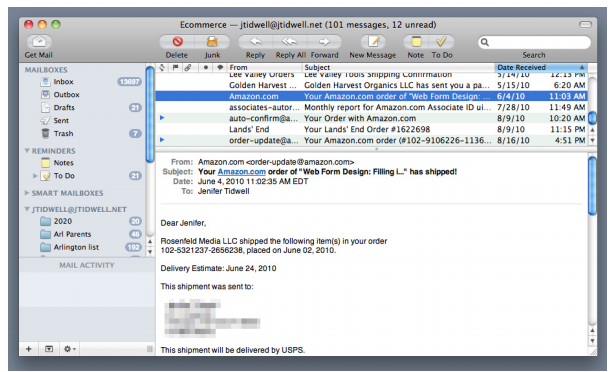
\includegraphics[scale=0.6]{images/lec07-pic50.png}
	\end{figure}
\end{frame}	

\begin{frame}[t]{One-Window Drilldown}
	Отображение списка или меню элементов в одном окне. Когда пользователь выбирает элемент из
списка, покажите детали или содержимое этого элемента в окне, заменив список.
	\begin{figure}[h]
		\centering
		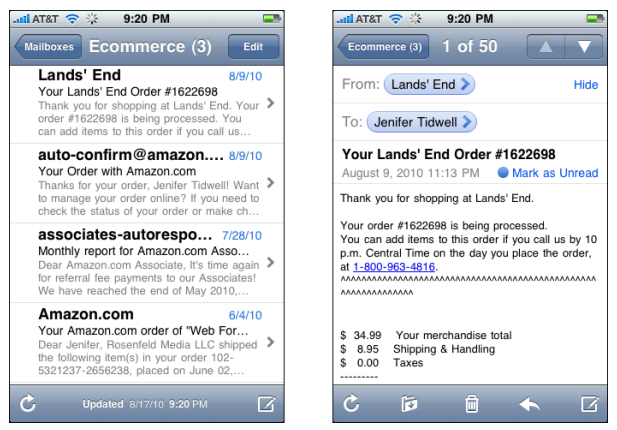
\includegraphics[scale=0.5]{images/lec07-pic51.png}
	\end{figure}
\end{frame}	

\begin{frame}[t]{List Inlay}
	Отображение списка элементов в виде строк в столбце. Когда пользователь выбирает элемент, откройте сведения об этом элементе на месте, в самом списке. Разрешите открывать и закрывать элементы независимо друг от друга.
	\begin{figure}[h]
		\centering
		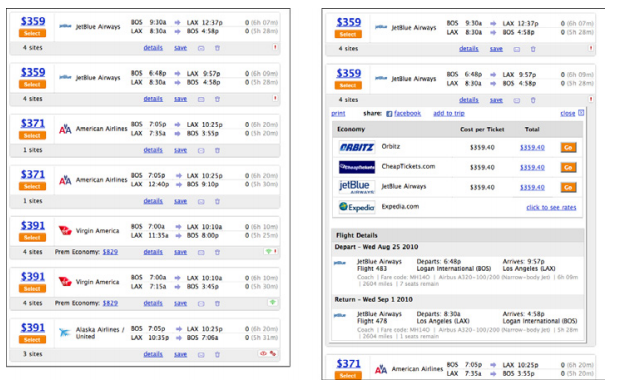
\includegraphics[scale=0.5]{images/lec07-pic52.png}
	\end{figure}
\end{frame}	

\begin{frame}[t]{List Inlay}	
	\begin{figure}[h]
		\centering
		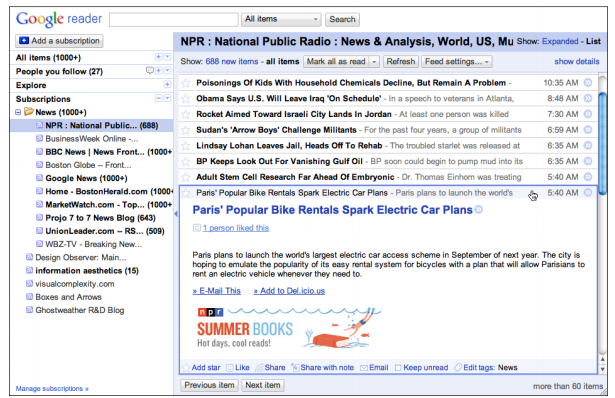
\includegraphics[scale=0.6]{images/lec07-pic53.png}
	\end{figure}
\end{frame}	

\begin{frame}[t]{Thumbnail Grid}
	Организуйте список визуально интересных элементов в сетку из миниатюрных изображений. Позвольте пользователю выбрать один или несколько эскизов для просмотра или управления этими элементами.
	\begin{figure}[h]
		\centering
		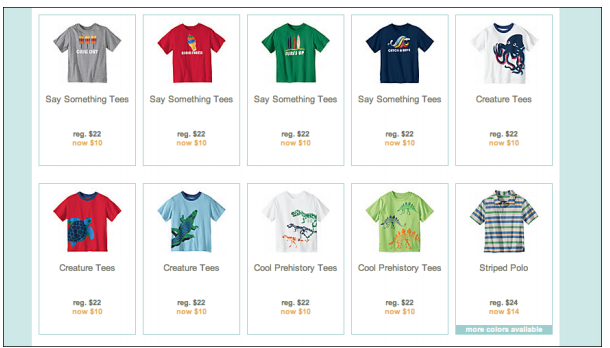
\includegraphics[scale=0.5]{images/lec07-pic54.png}
	\end{figure}
\end{frame}	

\begin{frame}[t]{Thumbnail Grid}
	\begin{figure}[h]
		\centering
		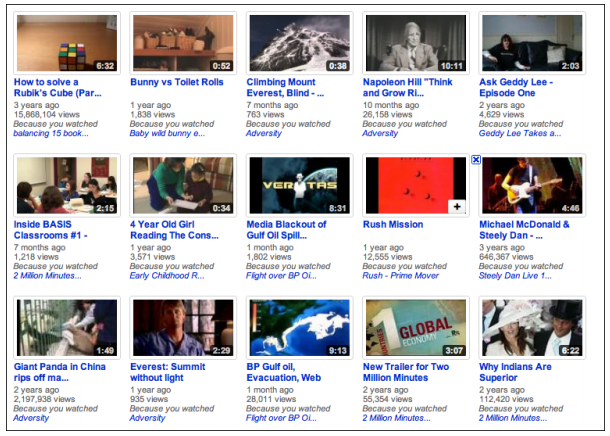
\includegraphics[scale=0.5]{images/lec07-pic55.png}
	\end{figure}
\end{frame}	

\begin{frame}[t]{Thumbnail Grid}
	\begin{figure}[h]
		\centering
		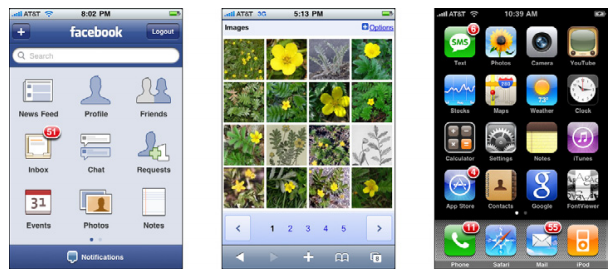
\includegraphics[scale=0.6]{images/lec07-pic56.png}
	\end{figure}
\end{frame}	

\begin{frame}[t]{Carousel}
	Расположите список визуально интересных элементов в виде горизонтальной полосы или дуги и позвольте пользователю
прокручивать или прокручивать миниатюры изображений. Увеличьте центральный элемент, если это необходимо.
	\begin{figure}[h]
		\centering
		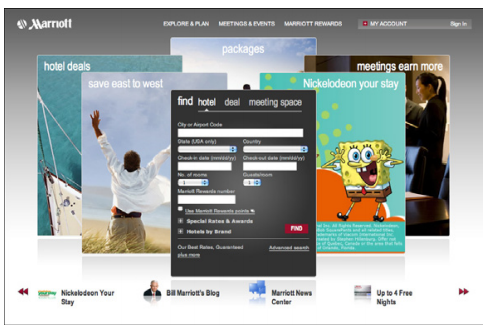
\includegraphics[scale=0.5]{images/lec07-pic57.png}
	\end{figure}
\end{frame}	

\begin{frame}[t]{Carousel}
	\begin{figure}[h]
		\centering
		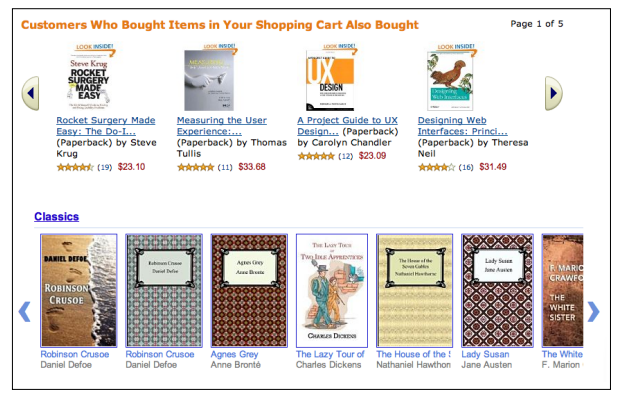
\includegraphics[scale=0.5]{images/lec07-pic58.png}
	\end{figure}
\end{frame}	

\begin{frame}[t]{Carousel}
	\begin{figure}[h]
		\centering
		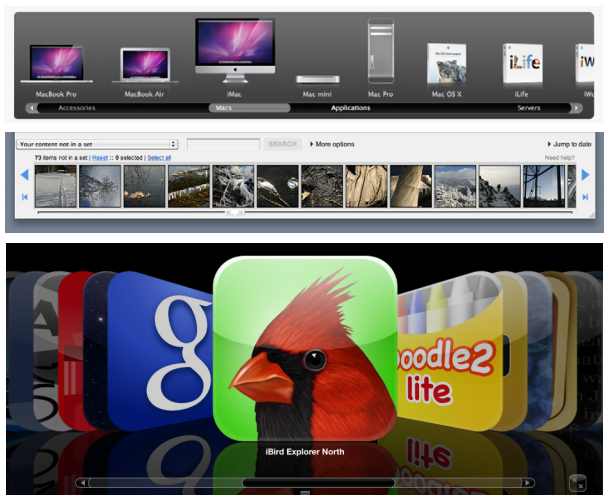
\includegraphics[scale=0.5]{images/lec07-pic59.png}
	\end{figure}
\end{frame}	

\begin{frame}[t]{Row Striping}
	Используйте два похожих оттенка для попеременного окрашивания фона строк таблицы
	\begin{figure}[h]
		\centering
		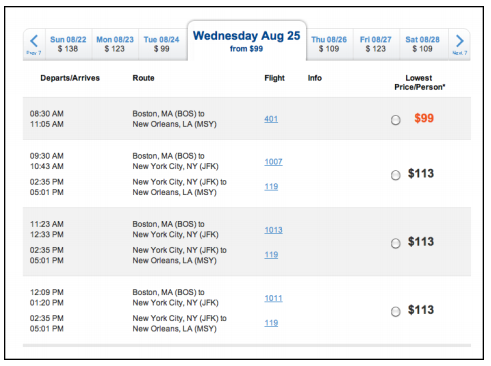
\includegraphics[scale=0.5]{images/lec07-pic60.png}
	\end{figure}
\end{frame}	

\begin{frame}[t]{Pagination}
	Разбейте очень длинный список на страницы и загружайте их по одной. Предоставьте пользователю элементы управления для навигации по списку --следующая, предыдущая, первая и последняя страницы.
	\begin{figure}[h]
		\centering
		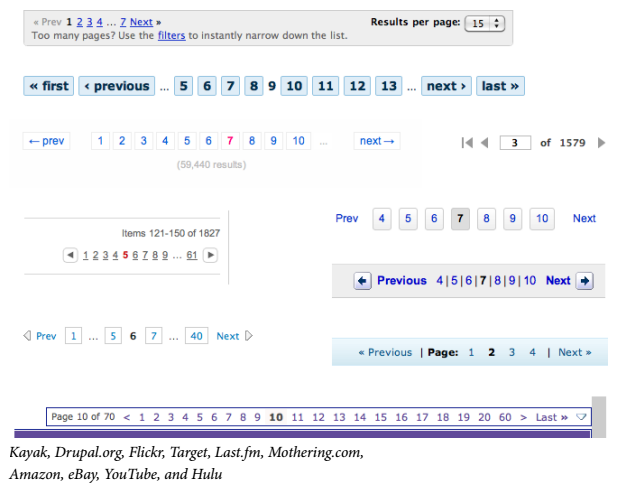
\includegraphics[scale=0.5]{images/lec07-pic62.png}
	\end{figure}
\end{frame}	

\begin{frame}[t]{Jump to Item}
	Когда пользователь вводит имя элемента в таблицу или дерево, перейдите прямо к этому элементу и выберите его.
	\begin{figure}[h]
		\centering
		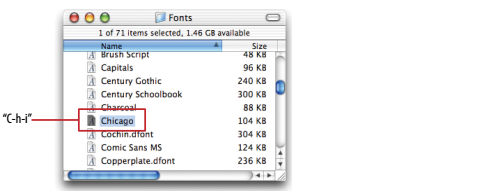
\includegraphics[scale=0.75]{images/lec07-pic63.png}
	\end{figure}
\end{frame}	

\begin{frame}[t]{Alphabet Scroller}
	Отобразите буквы алфавита, расположенные вдоль полосы прокрутки алфавитного списка.
	\begin{figure}[h]
		\centering
		\includegraphics[scale=0.5]{images/lec07-pic64.png}
	\end{figure}
\end{frame}	

\begin{frame}[t]{Cascading Lists}
	Отобразите иерархию, показав выбираемые списки элементов на каждом уровне иерархии.
	\begin{figure}[h]
		\centering
		\includegraphics[scale=0.5]{images/lec07-pic65.png}
	\end{figure}
\end{frame}	

\begin{frame}[t]{Tree-Table}
	Поместите поля элементов в столбцы таблицы, используйте структуру с отступом в первом столбце, чтобы проиллюстрировать древовидную структуру.
	\begin{figure}[h]
		\centering
		\includegraphics[scale=0.5]{images/lec07-pic66.png}
	\end{figure}
\end{frame}	

%\section{Расположение элементов}
%\section{Действия и команды}
%\section{Формы и элементы управления}

\end{document}
